\chapter{Implementation of the Game}
``Space-run'' was developed using the Godot Engine (version v3.2.3.stable) , an open-source game engine licensed under the MIT license. It is a cross-platform tool that offers a range of features for game development, including a visual scripting language, 2D and 3D graphics support, and a powerful physics engine. The Godot Engine utilizes a node-based architecture, where nodes are organized within scenes that can be reused, instanced, inherited, and nested. This structure allows for efficient project management and development within the engine. The game was written entirely in GDScript, the primary scripting language of the Godot Engine. Overall, the Godot Engine provides a user-friendly environment for game development and offers a comprehensive set of features for creating immersive and engaging games.

In addition to using the Godot Engine, the development team also utilized Blender (version 6.2.0) for creating and animating the characters in the game. Blender is a popular open-source 3D modeling and animation software that offers a range of features for creating detailed and realistic characters. The characters were then imported into the Godot Engine using the .glTF 2.0 file format, which is a widely supported file format for exchanging 3D graphics data.

\section{The top-level organization}
\begin{figure}[h]
    \centering
    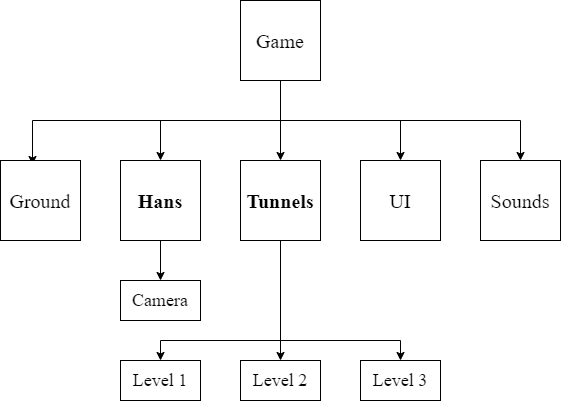
\includegraphics[width=0.8\textwidth]{game_tree}
    \caption{Structure of Game.tscn}
    \label{fig:game_tree}
\end{figure}

The main scene for the game, referred to as \texttt{Game.tscn}, is depicted in Figure \ref{fig:game_tree}. It includes several nodes, including Ground, UI, Sound, Game, Hans, and Tunnels. The Ground node is a CSGBox that serves as the ground in the game, while the UI and Sound nodes handle the user interface and audio aspects, respectively. The Game, Hans, and Tunnels nodes contain the majority of the game's functionality. Specifically, the Game node manages the overall gameplay, the Hans node controls the player character, and the Tunnels node manages the movement and appearance of the tunnels.

For a more in-depth understanding, let us examine some of the core aspects of the game in the following sections.

\section{Game}
The script for the Game node is the initial point of the game session and includes both the \texttt{\_start()} and \texttt{\_game\_over()} methods. It also serves as a link between the game and the agent environment described in Chapter \ref{agent_code_chapter}, and as such includes all of the necessary set methods for the agent environment. These methods allow for communication between the game and the agent environment, enabling the agent to interact with and influence the game.

The following examples demonstrate the simplified code of the main functions within \texttt{Game.gd}. It is important to note that code that is not relevant to any agent except the Keyboard agent, which is the player agent and the only one not designated as a "self-playing agent," has been omitted (and will be in future examples) as it is not relevant to the focus of this thesis. The Keyboard agent allows the player to interact with and control the game, while the other agents, referred to as "self-playing agents," operate independently within the game environment.

\begin{lstlisting}
func _ready():
    # lines relevant to the Keyboard agent:
    		...
    hans.set_speed(num_of_speed_ups)
    hans.set_tunnel_vars(starting_level, tunnel)  
    _start()
\end{lstlisting}

The ready function is called at the start of the game's execution and, after setting up the environment, it triggers the start function. This function initiates the gameplay and sets the necessary conditions for the game to proceed.

\begin{lstlisting}
func _start():
	# add all of obstacle objects specified in the environment
    for name in traps:
        tunnels.scenes["trap_scenes"].append(load("res://Scenes/Traps/" + name + ".tscn"))
        
    for name in bugs:
        tunnels.scenes["bug_scenes"].append(load("res://Scenes/Characters/Bugs/" + name + ".tscn"))
        
    for name in viruses:
        tunnels.scenes["virus_scenes"].append(load("res://Scenes/Characters/Viruses/" + name + ".tscn"))
        
    for name in tokens:
        tunnels.scenes["token_scenes"].append(load("res://Scenes/Tokens/" + name + ".tscn"))
    
    # set Hans's position in front of the chosen tunnel
    match tunnel:
        hans.lvl.TWO:
            hans.translation = Vector3(1250,-32,0)
        hans.lvl.THREE:
            hans.translation = Vector3(-1250,-32,0)
    
    # add traps to the first tunnel Hans is passing through
    tunnels.create_first_level_traps(tunnel)
\end{lstlisting}  

As described in more detail in Chapter \ref{agent_code_chapter}, the user can specify environment parameters and a starting level for the agent through the command line. These parameters determine the obstacles that the player will face and the starting position of the player character, Hans. The start function incorporates these parameters into the obstacle arrays and positions Hans accordingly. The function also generates the obstacles for the designated starting level. The creation and deletion of obstacles during gameplay is discussed in Section \ref{tunnel_script} of this chapter.

\begin{lstlisting} 
func _game_over():
    if DEBUG:
    		# print debugging statement
        print('died on level %d, rot = %d' % [level.level, state.state[1]])
    if self_playing_agent:
    		# if this is an agent playing, emit the necesarry signal that the game is over
        emit_signal("game_finished", score.get_score(), num_of_ticks, level.get_level() > max_tunnels, OS.get_ticks_msec() / 1000.0) 
        queue_free()
    else:
    		# otherwise handle the game over for the player
        
\end{lstlisting}

The game over function manages the end of the game and sends a signal to the top-level script, \texttt{Main.gd} (described in Chapter \ref{agent_code_chapter}), indicating that the game has ended. It also provides \texttt{Main.gd} with the necessary information about the game's status and outcome.

\section{Hans}
The next node we want to examine is Hans. While \texttt{Hans.tscn} is a scene with the main character and its necesarry animations, what interests us more is the Hans.gd and its key components.

\begin{lstlisting}
func _physics_process(delta): 
	# code used to update the variables and UI
		...
			
    tunnels.delete_obstacle_until_x(curr_tunnel,translation.x - tunnels_children[curr_tunnel].translation.x + 50)
    
    # create a trap in the next tunnel every 50 meters
    if translation.x < new_trap:
        create_new_trap()
    
    # updating score 
    score._on_Meter_Passed()
    
    # Hans's movement
    var velocity = Vector3.LEFT * speed
    velocity = move_and_slide(velocity)
    
    # in case Hans colided with somehting, handle it properly
    check_collisions()
    
    # bugs and viruses need to move torwards Hans    
    tunnels.bug_virus_movement(delta, curr_tunnel)
    
    if isShootingButtonPressed:
        shoot()
        
    # type needs to be calculated before 
    # so we know where the next trap is on x axis
    var type = calc_type()
    state.update_state(calc_dist(),calc_rot(),type)
\end{lstlisting}

The primary function within \texttt{Hans.gd} is the \texttt{\_physics\_process()}, which is called on every tick of the game. It handles the main aspects of the player character through the use of various methods and functions. These include deleting passed obstacles, creating new obstacles every 50 meters, updating the score, handling the movement of the player character, bugs and viruses, and determining the current state of the player. The state label, which is displayed on the upper right corner of the screen (as shown in Figure \ref{fig:third_tunnel}), is the primary information that agents receive when making decisions about their next move, as described in Chapter \ref{agent_code_chapter}. The \texttt{\_physics\_process()} function also handles collisions and shooting if the player chooses to do so. Overall, this function plays a crucial role in the gameplay and management of the player character.

It is also worth noting that this script handles the movement of the tunnels to the back as Hans passes them, with the first tunnel being moved to be after the third one. This feature allows for the game to be infinite, as the tunnels are constantly cycled and reused.

\begin{figure}[h]
    \centering
    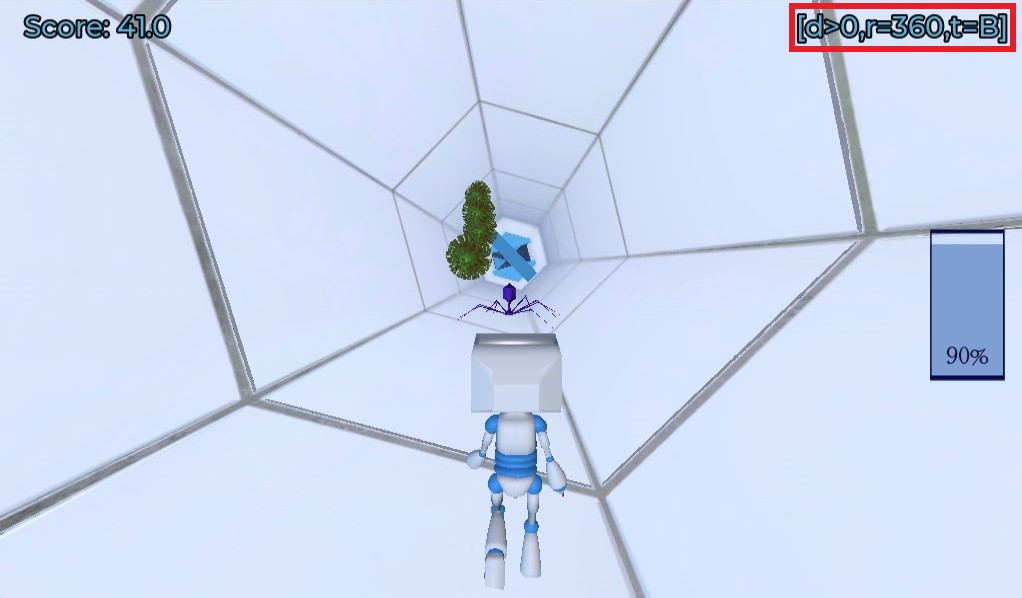
\includegraphics[width=\textwidth]{third_tunnel}
    \caption{State}
    \label{fig:third_tunnel}
\end{figure}

\section{Tunnels}
\label{tunnel_script}
The Tunnels node, which is a child of the main scene in the game tree, contains three child nodes of the Spatial type (level1, level2, and level3) and each of these nodes includes a CSGTorus node, which represents the physical appearance of the tunnels. Obstacles are added to the appropriate level node as instances. The \texttt{Tunnels.gd} script, which is attached to the Tunnels node, handles many of the previously mentioned functions such as obstacle creation and deletion and tunnel rotation. In the following code snippets, we will examine the Tunnels.gd script in greater detail.

\begin{lstlisting}
func _physics_process(delta):   
	# gets move from the agent
	# in case we chose the Keyboard agent 
	#this will just return input from the keyboard
    var move = game.agent.move(game.state.get_state(), game.score.get_score(), game.num_of_ticks)
    
    #rotates the tunnel
    if move[0] == 1:
        var tunnel = get_child(hans.get_current_tunnel())
        tunnel.rotate_object_local(Vector3.RIGHT,-ROTATE_SPEED * delta)
    elif move[0] == -1:
        var tunnel = get_child(hans.get_current_tunnel())
        tunnel.rotate_object_local(Vector3.LEFT,-ROTATE_SPEED * delta)
        
    # shoot if necesarry
    if not hans == null: # if it is not instanced we can't call the function       
        hans.switch_animation(move[1] == 1)
\end{lstlisting}

The \texttt{\_physics\_process()} function within the \texttt{Tunnels.gd} script serves as the primary connection between the agent and the game. As shown in the provided code, the function retrieves the next move from the agent and rotates the tunnel accordingly, potentially including shooting as well.

\begin{lstlisting} 
func create_first_level_traps(tunnel):
    # get the level we are making traps for
    var level = tunnel
    
    # pick number of traps to be added
    var num_of_traps = rand.randi_range(50,65)
    var x = 1200
    
    for n in num_of_traps:
        # add space between traps
        x -= rand.randi_range(TRAP_RANGE_FROM,TRAP_RANGE_TO)
        # check if the trap will be inside the tunnel
        # if not, break
        if x < -1200:
            break
        create_one_obstacle(level, x) 
\end{lstlisting}

The function depicted in the code above serves to generate obstacles in the starting tunnel. By periodically creating traps in the tunnel ahead, the game is able to prevent lag caused by an excessive number of objects existing simultaneously. For that reason, this function is used only once, at the beginning of the game.

\begin{lstlisting} 
func create_one_obstacle(level,x):
    # pick which kind of obstacle will be added
    # this process is partially random, depending on weather the tunnel 
    # can contain one or more kinds of obstacles
    var scene  = pick_scene(level)   
    
    # get the level we are making traps for
    var tunnel = get_child(level)
    
    # randomly pick an obstacle
    var i = pick_obstacle(scene)
    
    # make an instance
    var obstacle = scene[i].instance()
    obstacle.translation.x = x
    
    tunnel.add_child(obstacle)
    
    # randomly pick obstacle rotation
    rotate_obstacle(obstacle)
\end{lstlisting}

The tunnels are positioned along the x axis, and this function allows for the creation of obstacles within them at specific x positions.

\begin{lstlisting}           
func delete_obstacle_until_x(level,x):
    var tunnel = get_child(level)
    # loop through children of the tunnel
    # and eliminate any obstacles
    # until position x
    for obstacle in tunnel.get_children():
        if not "light" in obstacle.name and not "torus" in obstacle.name and not "Bullet" in obstacle.name:
            if obstacle.translation.x > x:
                obstacle.queue_free()
            else:
                return
\end{lstlisting}

As previously mentioned, by dynamically deleting passed obstacles, the game is able to maintain a stable performance and avoid overloading the system. The provided code demonstrates the implementation of this function.
